\documentclass{llncs}

%\usepackage[margin=1in]{geometry}
\usepackage{amsmath, amssymb, mathtools}
\usepackage{enumitem}
\usepackage{float}
\usepackage{hyperref}
\usepackage{listings}
\usepackage{graphicx}

\def\labelitemi{$\bullet$}
\def\labelenumi{(\textbf{\arabic{enumi}})}

\usepackage{tikz}
\usetikzlibrary{trees}

\newcounter{algo}

\floatstyle{ruled}
\newfloat{algo}{h}{aux}
\floatname{algo}{Algorithm}

\input preamble

\begin{document}

\title{Linear Reduction: Parsing and Interpreting Code Without Trees}
\author{Ari Feiglin\inst{1}\and Dr. Yoni Zohar\inst{1}}
\institute{University of Bar Ilan, Ramat Gan, Israel}

\maketitle

\begin{abstract}

    In this paper we discuss an alternative method to parsing and interpreting human-readable code.
    This method utilizes an iterative approach, as opposed to a recursive tree-oriented approach found in most modern compilers and interpreters.
    We will implement our algorithm in an interpreter and compare it with an interpreter created using more classical means.

    \keywords{Parsing \and Interpreting \and AST \and Parse Trees}

\end{abstract}

\section{Introduction}

Nowadays, most programming language interpreters follow the following pipeline:
\begin{enumerate}
    \item Lexing: lexically analyze the input code, separating it into atomic \textit{tokens}.
    \item Parsing: convert the parsed tokens into a \textit{parse tree}: a tree which represents the grammar of the code.
    \item Interpreting: recursively descend the tree and execute the code according to the instructions embedded in the tree.
\end{enumerate}
For example, we can parse the following expression:

\centerline{\texttt{1 + 2 * 3 + 4}}

\noindent as follows

\medskip
\centerline{\begin{tikzpicture}
\node{\texttt{+}}
child {node {\texttt{1}}}
child {node {\texttt{+}}
    child {node {\texttt{*}}
        child {node {\texttt{2}}}
        child {node {\texttt{3}}}
    }
    child {node {\texttt{4}}}
};
\end{tikzpicture}}
\medskip

One can then descend the parse tree and compute the expression.
Explicitly, if you reach a node whose operator is $\circ$, evaluate the left tree to get $x$, evaluate the right tree to get $y$, and then return $x\circ y$.

Unfortunately, constructing such a tree is not so easy.
Multiple methods for doing so exist, as well as tools for automating this process.

We will propose a novel method for the process of interpretation, which doesn't use parse trees.
Parsing code generated by context-free grammars (CFGs) is inherently a recursive process, and thus it is not surprising that our algorithm can be altered to instead produce parse trees.

\section{Notation}

\begin{enumerate}
    \item $\bN$ denotes the set of natural numbers, including $0$.
    \item $\bbN$ is defined to be $\bN\cup\set\infty$.
    \item $\bZ$ denotes the set of integer numbers.
    \item $\bbZ$ is defined to be $\bZ\cup\set{\pm\infty}$.
    \item $f\colon A\partial B$ means that $f$ is a partial function from $A$ to $B$ (i.e. $\operatorname{dom}f\subseteq A$).
    \item $\epsilon$ denotes the empty string.
    \item If $\mathcal L$ is a language (a set of strings), then $\mathcal L^\epsilon$ is equal to $\mathcal L\cup\set\epsilon$.
    \item A list is denoted by $(x_1,\dots,x_n)$.
    \item The concatenation of two lists $\ell_1$ and $\ell_2$ is denoted by $\ell_1@\ell_2$.
    \item $x::\ell$ is the list whose first element is $x$ and tail is $\ell$.
\end{enumerate}

\section{The Algorithm}

\subsection{A First Attempt -- Primitive Reduction}

The idea of the algorithm is as follows: given a string of tokens $\mb{\sigma^1}\cdots\mb{\sigma^n}$ (for readability, tokens are written in boxes), we form rules for combining two tokens.
For example $\mb{\ttt1}$ and $\mb{\ttt+}$ can be combined together to give a token $\mb{\ttt{1,+}}$.
Then if we follow a token of the form $\mb{\ttt{x,+}}$ with a token of the form $\mb{\ttt y}$, the tokens are combined to form a token $\mb{\ttt{x+y}}$.
So for example:
\[ \mbt{1} \mbt{+} \mbt{2} \mbt{+} \mbt{3} \to \mbt{1,+} \mbt2 \mbt+ \mbt3 \to \mbt{3} \mbt+ \mbt3 \to \mbt{3,+} \mbt3 \to \mbt6 \]
But what about \ttt{1+2*3}?
We'd get
\[ \mbt1 \mbt+ \mbt2 \mbt* \mbt3 \to \mbt{1,+} \mbt2 \mbt* \mbt3 \to \mbt3 \mbt* \mbt3 \to \mbt{3,*} \mbt3 \to \mbt9 \]

So to remedy this we add the concept of \textit{priorities}: for each symbol in our alphabet $\Sigma$, we assign a priority $p\in\bbN$.
This can be thought of as a \textit{priority function} $\pi\colon\Sigma\longto\bbN$.
So if the tokens $\mb{\sigma^1}\cdots\mb{\sigma^n}$ have respective priorities $p_1,\dots,p_n$ we can form the string $\mb{\sigma^1}_{p_1}\cdots\mb{\sigma^n}_{p_n}$ (where the subscript is part of the
character).
Now, we only combine two tokens if the token of the first is at least as great as the token of the second, and then the combined token gets the lower (the second) of the two priorities.
So we can assign to tokens containing numbers a priority of $\infty$, the token \ttt+ gets a priority of $1$, and $\ttt*$ gets a priority of $2$.
Then this becomes:
\[ \mbt1_\infty \mbt+_1 \mbt2_\infty \mbt*_2 \mbt3_\infty \to \mbt{1,+}_1 \mbt2_\infty \mbt*_2 \mbt3_\infty \to \mbt{1,+}_1 \mbt{2,*}_2 \mbt3_\infty \]
This cannot be combined any further, so we need another rule: we will give the final token a priority of $0$, so this becomes:
\[ \mbt{1,+}_1 \mbt{2,*}_2 \mbt3_0 \to \mbt{1,+}_1 \mbt{6}_0 \to \mbt{7}_0 \]
which is the correct result.

We can formalize this as follows: we start with an alphabet $\Sigma$.
Define $\oS=\Sigma\times\bbN$, and we define a so-called \textit{initial $\beta$-reducer}: $\hb\colon \Sigma\times\Sigma \longto \Sigma$.
This is a function which tells us how to combine tokens together.
And we extend it to a \textit{derived $\beta$-reducer} which is a function $\beta\colon\oS^*\longto\oS^*$ as follows.

Suppose $\xi=\sigma^1_{p_1}\cdots\sigma^n_{p_n}$, then $\beta(\xi)$ is defined recursively as follows:
\begin{enumerate}
    \item if $n=1$, then $\beta(\xi)=\sigma^n_0$,
    \item if $p_1\geq p_2$, then $\beta(\xi)=\hb(\sigma^1,\sigma^2)_{p_2}\sigma^3_{p_3}\cdots\sigma^n_{p_n}$,
    \item otherwise $\beta(\xi)=\sigma^1_{p_1}\,\beta(\sigma^2_{p_2}\cdots\sigma^n_{p_n})$.
\end{enumerate}

Notice that we need to add extra rules, like $\beta(\mbt{x,*},\mbt{y,+})=\mbt{x*y,+}$.
This is so we can handle
\begin{multline*}
    \mbt1_\infty \mbt*_2 \mbt2_\infty \mbt+_1 \mbt3_\infty \to \mbt{1,*}_2 \mbt2_\infty \mbt+_1 \mbt3_\infty \to \mbt{1,*}_2 \mbt{2,+}_1 \mbt3_\infty \to \mbt{2,+}_1 \mbt3_\infty\\
    \to \mbt{2,+}_1 \mbt3_0 \to \mbt5_0
\end{multline*}

But this has a major issue: it can't handle things like parentheses.
So we need to come up with a second attempt.

\subsection{A Second Attempt -- Partial Reduction}

In order to handle parentheses, all we need to do is to make a simple change to our algorithm.
Instead of a full function which also tells us how to compute the new priority, the initial $\beta$-reducer will be a partial function:
\[ \hb\colon \Sigma\times\Sigma\partial\Sigma\times(\bbZ\times\bbZ\to\bbZ) \]
Now we define the derived $\beta$-reducer as follows; it is a function $\beta\colon\oS^*\partial\oS^*$ where for $\xi=\sigma^1_{p_1}\cdots\sigma^n_{p_n}$:
\begin{enumerate}
    \item if $n=1$ then $\beta(\xi)=\sigma^n_0$,
    \item if $p_1\geq p_2$ and $\hb(\sigma^1,\sigma^2)=(\tau,\rho)$ is defined, then $\beta(\xi)=\tau_{\rho(p_1,p_2)}\sigma^3_{p_3}\cdots\sigma^n_{p_n}$,
    \item otherwise $\beta(\xi)=\sigma^1_{p_1}\,\beta(\sigma^2_{p_2}\cdots\sigma^n_{p_n})$.
\end{enumerate}

Now we define our initial $\beta$-reducer which will support parentheses.
It is an extension of our previous $\beta$-reducer:
\begin{gather*}
    \hb(\mbt x,\mb\circ) = (\mb{\ttt x,\circ},\snd),\quad \hb(\mb{\ttt x,\circ},\mbt y) = (\mb{\ttt x\circ\ttt y},\snd) \qquad \hbox{for $\circ\in\set{\ttt{+,*}}$} \\
    \hb(\mbt{x,*},\mbt{y,+}) = (\mbt{x*y,+},\snd)
\end{gather*}
where $\fst,\snd$ are the first and second projections, respectively (i.e. $(x,y)\mapsto x$ and $(x,y)\mapsto y$).
We then add the rules for parentheses:
\begin{gather*}
    \hb(\mbt x,\mbt)) = (\mbt{x,)},\snd),\quad \hb{\mb{\ttt x,\circ},\mbt{y,)}} = (\mb{\ttt x\circ\ttt y,\ttt)},\snd) \qquad \hbox{for $\circ\in\set{\ttt{+,*}}$} \\
    \hb(\mbt(,\mbt{x,)}) = (\mbt x,\fst)
\end{gather*}
\gobble) % syntax highlighting
And we define our priority function as follows:
\[ \pi(\mbt x) = \infty\hbox{ for numbers \ttt x},\quad \pi(\mbt+) = 1,\quad \pi(\mbt*) = 2,\quad \pi(\mbt() = \infty,\quad \pi(\mbt)) = 0 \]

Now take for example \ttt{2*(1+3)+4}:
\begin{align*}
    \mbt2_\oo \mbt*_2 \mbt(_\oo \mbt1_\oo \mbt+_1 \mbt3_\oo \mbt)_0 \mbt+_1 \mbt4_\oo &\to \mbt{2,*}_2 \mbt(_\oo \mbt1_\oo \mbt+_1 \mbt3_\oo \mbt)_0 \mbt+_1 \mbt4_\oo\\
        &\to \mbt{2,*}_2 \mbt(_\oo \mbt{1,+}_1 \mbt3_\oo \mbt)_0\mbt+_1 \mbt4_\oo\\
        &\to \mbt{2,*}_2 \mbt(_\oo \mbt{1,+}_1 \mbt{3,)}_0 \mbt+_1 \mbt4_\oo\\
        &\to \mbt{2,*}_2 \mbt(_\oo \mbt{4,)}_0 \mbt+_1 \mbt4_\oo\\
        &\to \mbt{2,*}_2 \mbt4_\oo \mbt+_1 \mbt4_\oo\\
        &\to \mbt{2,*}_2 \mbt{4,+}_1 \mbt4_\oo\\
        &\to \mbt{8,+}_1 \mbt4_\oo\\
        &\to \mbt{8,+}_1 \mbt4_0\\
        &\to \mbt{12}_0
\end{align*}
\gobble)\gobble)

Notice that our $\beta$-reducers don't care about the exact value of the number and operation: both $\mbt1\mbt+$ and $\mbt2\mbt*$ are mapped to something of the form $\mbt{x,$\circ$}$.
We can thus abstract away the exact value of tokens and have our initial $\beta$-reducer deal only with the form of the token.
We do such in our third attempt.

\subsection{A Third Attempt -- Valued Reduction} \label{valued-reduction}

Here we will abstract away the value of each term; the value of the new term given by the initial $\beta$-reducer will be determined by an output function.
Our alphabet of types $\Sigma$, instead of having a token for every number, will just have tokens for types (number, operator, etc.).
We will also have another set $\values$, the \textit{universe of values}.

The initial $\beta$-reducer is a function
\[ \hb \colon \Sigma\times\Sigma \partial \Sigma\times(\bbZ\times\bbZ\to\bbZ)\times(\values\times\values\partial\values) \]
Our alphabet of types is $\Sigma=\set{\NUM,\OP,\LPAREN,\RPAREN,\OP\NUM,\RPAREN\NUM}$, define $\oP=\oS\times\values$ to be the set of all possible terms (which is a type, a priority, and a value).
Since terms now consist of three parts, we write them as $\sigma_p(v)$, where $\sigma$ is the type; $p$ is the priority; and $v$ the value.

Our rules for the derived $\beta$-reducer is similar to before: it is a function $\beta\colon\oP^* \partial \oP^*$ where for $\xi=\sigma^1_{p_1}(v_1)\cdots\sigma^n_{p_n}(v_n)$
\begin{enumerate}
    \item if $n=1$ then $\beta(\xi)=\sigma^n_0(v_n)$,
    \item if $p_1\geq p_2$ and $\hb(\sigma^1,\sigma^2)=(\tau,\rho,f)$ is defined, then
    \[ \beta(\xi)=\tau_{\rho(p_1,p_2)}(f(v_1,v_2))\sigma^3_{p_3}(v_3)\cdots\sigma^n_{p_n}(v_n) \]
    \item otherwise $\beta(\xi)=\sigma^1_{p_1}(v_1)\beta(\sigma^2_{p_2}(v_2)\cdots\sigma^n_{p_n}(v_n))$.
\end{enumerate}

Our initial $\beta$-reducer will is defined as follows:
\begin{itemize}
    \item $\hb(\NUM,\OP)=(\OP\NUM,\snd,(v,f\mapsto(v,f))$
    \item $\hb(\OP\NUM,\NUM)=(\NUM,\snd,((v,f),u\mapsto f(v,u)))$
    \item $\hb(\OP\NUM,\OP\NUM)=(\OP\NUM,\snd,((v,f),(u,g)\mapsto (f(v,u),g))$
    \item $\hb(\NUM,\RPAREN)=(\RPAREN\NUM,\snd,(v,\_\mapsto v))$
    \item $\hb(\OP\NUM,\RPAREN\NUM)=(\RPAREN\NUM,\snd,((v,f),u\mapsto f(v,u)))$
    \item $\hb(\LPAREN,\RPAREN\NUM)=(\NUM,\fst,(\_,v\mapsto v))$
\end{itemize}

But this of course is not capable of handling the semantics necessary for programming languages.
We need a notion of a state, and a somewhat more refined algorithm.

\subsection{A Fourth Attempt -- Stateful Reduction}

We define the following four base sets:
\begin{enumerate}
    \item $\values$ the \textit{universe of values}; these are all the internal values an object may have.
    \item $\termp$ the set of \textit{printable terms}; this is the set of all printable tokens a programmer may type.
    \item $\terms$ the set of \textit{type terms}; these are terms which correspond to types in the classical sense.
    \item $\terma$ the set of \textit{abstract terms}; these are intermediate terms (like $\OP\NUM$ from the previous section).
\end{enumerate}
The sets $\termp,\terms,\terma$ are disjoint, and we place no such restriction on $\values$.

While we don't need to place any further restrictions on $\termp,\terms,\terma$, we found it useful to explicitly construct them.
To construct $\terms$, we begin with a set of \textit{base types} $\Sigma$.
Each base type has an associated arity in $\bbN$; let $\Sigma^n$ denote the set of all base types of arity $n$.
Then we define $\terms$ as follows:
\[ \terms \ccoloneqq \Sigma^0 \mid \Sigma^1\terms \mid \Sigma^2\terms\terms \mid \Sigma^3\terms\terms\terms \mid \cdots \mid \Sigma^\oo(\terms\cdots\terms) \]

To construct $\terma$ we start with $\mathcal A$, a set of \textit{atomic abstract terms}, again each with an arity in $\bbN$.
$\mathcal A^n$ is the set of atomic abstract terms of a set arity $n$.
Then $\terma$ is defined by
\[ \terma \ccoloneqq \mathcal A^0\mid\mathcal A^1\terms^\epsilon\mid\mathcal A^2\terms^\epsilon\terms^\epsilon\mid\mathcal A^3\terms^\epsilon\terms^\epsilon\terms^\epsilon\mid\cdots\mid
\mathcal A^\infty\terms^\epsilon\cdots\terms^\epsilon \]
Here we allow inputs to atomic abstract terms to be empty (i.e. $\terms^\epsilon$ instead of just $\terms$).

So if $\Sigma=\set{\NUM_0,\LIST_1,\PRODUCT_\infty}$ (the subscripts are the arities of each base type) and $\mathcal A=\set{\OP}$, then
\[ \NUM,\LIST\NUM,\PRODUCT(\LIST\NUM\NUM)\in\terms,\qquad \OP\LIST\NUM\in\terma \]
For readability we can put parentheses and commas where necessary, but importantly these sets have the \textit{unique reconstruction property}: it is possible to compute their construction from the
string itself (i.e. a string cannot be constructed from two different patterns).

Now we define the following sets:
\begin{enumerate}
    \item $\term=\termp\cup\terms\cup\terms$, the set of \textit{terms},
    \item $\termi=\terms\cup\terma$, the set of \textit{internal terms},
    \item $\expi=\termi\times\values$, the set of \textit{internal expressions},
    \item $\exp=\termi\cup\termp$, the set of \textit{expressions}.
\end{enumerate}
Finally we define $\oe=\exp\times\bbZ$.
Elements of $\oe$ will be written like $\sigma_n(v)$ as before; for printable terms we act as if the value is empty.

The \textit{initial priority function} is a function $\pi\colon\termp\longto\bbZ$.
This can be naturally extended to $\pi\colon\termp^*\longto\oe^*$.

Finally, our \textit{initial $\beta$-reducer} is a function ($\state$ is a set of functions $\termp\partial\expi$ which we will define later)
\[ \hb\colon\termi\times\term^\epsilon \partial \termi^\epsilon\times(\bbZ\times\bbZ\to\bbZ)\times(\values\times\values\times\state\partial\values\times\termp^*\times\state) \]
and we extend this to a \textit{derived $\beta$-reducer}, a function
\[ \beta\colon\oe^*\times\state \partial \oe^*\times\state \]
inputs in $\oe^*\times\state$ will be written as $\gen\xi[\bar s]$ for $\xi\in\oe^*$ and $\bar s\in\state$.
We define $\beta^*\gen\xi[\bar s]$ to be the value obtained by composing $\beta$ with itself of $\gen\xi[\bar s]$ until the convergence of $\xi$.
Meaning
\begin{multline*}
    \beta^* = \beta^n\gen\xi[\bar s]\\
    \hbox{where $n=\min\set{n\geq1}[{\beta^n\gen\xi[\bar s]=\gen{\xi'}[\bar s'],\beta\gen{\xi'}[\bar s']=\gen{\xi'}[\bar s'']}]$}
\end{multline*}
We define $\beta\gen\xi[\bar s]$ as follows, where $\xi=\sigma^1_{p_1}(v_1)\cdots\sigma^n_{p_n}(v_n)$.
\begin{enumerate}
    \item if $\sigma^1\in\termp$ then
    \[ \beta\gen\xi[\bar s] = \gen{s(\sigma^1)_{p_1}\sigma^2_{p_2}(v_2)\cdots\sigma^n_{p_n}(v_n)}[\bar s] \]
    \item if $\hb(\sigma^1,\epsilon)=(\tau,\rho,f)$ is defined, then compute $f(v_1,\_,s)=(u,\xi',s')$ and $\beta^*\gen{\pi\xi'}[\bar s']=\gen{\xi''}[\bar s'']$, and
    \[ \beta\gen\xi[\bar s] = \gen{\tau_{\rho(p_1,\_)}\xi''\sigma^2_{p_2}(v_2)\cdots\sigma^n_{p_n}(v_n)}[\bar s''] \]
    \item if $p_1\geq p_2$ and $\hb(\sigma^1,\sigma^2)=(\tau,\rho,f)$ is defined, then compute $f(v_1,v_2,s)=(u,\xi',s')$ and $\beta^*\gen{\pi\xi'}[\bar s']=\gen{\xi''}[\bar s'']$, and
    \[ \beta\gen\xi[\bar s] = \gen{\tau_{\rho(p_1,p_2)}\xi''\sigma^3_{p_3}(v_2)\cdots\sigma^n_{p_n}(v_n)}[\bar s''] \]
    \item otherwise compute $\beta\gen{\sigma^2_{p_2}(v_2)\cdots\sigma^n_{p_n}(v_n)}[\bar s]=\gen{\xi'}[\bar s']$ and
    \[ \beta\gen\xi[\bar s] = \gen{\sigma^1_{p_1}(v_1)\xi'}[\bar s'] \]
\end{enumerate}

\subsubsection{States}

We begin by defining \textit{point-states} to be partial maps $\termp\partial\expi$.
If $s_1,s_2$ are two point-states then we define their composition to be
\[ s_1s_2(\sigma) = \begin{cases} s_2(\sigma) & \sigma\in\dom s_2\\ s_1(\sigma) & \sigma\in\dom s_1-\dom s_2\end{cases} \]
Point-states with finite domain will be denoted by $[\sigma_i\mapsto\varkappa_i]_{i=1}^n$ where $\sigma_1,\dots,\sigma_n$ is the domain and $\varkappa_1,\dots,\varkappa_n$ are their respective images.

A \textit{state} will be a pair of a sequence of point-states and a set of indices.
This will be denoted by $\bar s=[(s_1,\dots,s_n),\;I=(i_1,\dots,i_k)]$ (we require that $k\leq n$).
We define
\begin{enumerate}
    \item $\bar s+s=\bigl[(s_1,\dots,s_n,s),\;I\bigr]$, for $s$ a point-state,
    \item $\bar s+_cs=\bigl[(s_1,\dots,s_n,s),\;(i_1,\dots,i_k,n+1)\bigr]$, for $s$ a point-state,
    \item $\pop\bar s=\bigl[(s_1,\dots,s_{n-1}),\;I\bigr]$ if $i_k<n$, otherwise it is defined to be equal to $\bigl[(s_1,\dots,s_{n-1}),\;(i_1,\dots,i_{k-1})\bigr]$,
    \item $\bar ss=\bigl[(s_1,\dots,s_{n-1},s_ns),\;I\bigr]$ for $s$ a point-state,
    \item $\bar s(\sigma)=s_1\cdots s_n(\sigma)$ for $\sigma\in\termp$,
    \item $\bar s_c=s_{i_k}\cdots s_n$,
    \item if $\sigma\in\termp$ and $\varkappa\in\expi$ then $\bar s\{\sigma\mapsto\varkappa\}=\bigl[(s_1,\dots,s_k[\sigma\mapsto\varkappa],\dots,s_n),\;I\bigr]$ where $k$ is the maximum index such that
    $\sigma\in\dom s_k$.
\end{enumerate}

\section{Implementing the Algorithm}

We will implement our algorithm in an interpreter for a toy language we dubbed ``LLang''.
We will also create an interpreter for LLang using menhir\NEEDCITE{}.
In this section we will detail the implementation of our algorithm and compare and contrast the two implementations.

\subsection{The Grammar}

The grammar for our toy language is pretty straight-forward:

\medskip
\grammar
\noalign{\hbox{\bf Identifiers}}
    letter&\ccoloneqq\(a\dots z\gbar A\dots Z\gbar\_\)\cr
    digit&\ccoloneqq\(0\dots9\)\cr
    non\_digit&\ccoloneqq\(\_\gbar{\it letter}\)\cr
    ident&\ccoloneqq{\it letter}\ \({\it digit}\gbar{\it non\_digit}\)^*\cr
    pident&\ccoloneqq {\bf\_prim\_} \({\it digit}\gbar{\it non\_digit}\)^*\cr
\noalign{\hbox{\bf Constant Expressions}}
    const&\ccoloneqq\({\it number}\gbar{\it product}\)\cr
    number&\ccoloneqq\({\it digit}\)^*[.\({\it digit}\)^*]\cr
\noalign{\hbox{\bf Operators}}
    op&\ccoloneqq\(@\gbar+\gbar-\gbar*\gbar/\gbar{<=}\gbar{<}\gbar{>=}\gbar{>}\gbar{==}\gbar{!}{=}\)\cr
\noalign{\hbox{\bf Expressions}}
    expr&\ccoloneqq\epsilon\cr
        &\bbar{\bf let}\ {\it ident}\ =\ {\it value}\ ;\ {\it expr}\cr
        &\bbar{\bf fun}\ {\it ident}\ (\ {\it plist}\ )\ \{\ {\it expr}\ \}\ {\it expr}\cr
        &\bbar{\bf if}\ (\ {\it value}\ )\ \{\ {\it expr}\ \}\ \{\ {\it expr}\ \}\ {\it expr}\cr
        &\bbar{\it funcall}\ ;\ {\it expr}\cr
        &\bbar{\it pident}\ {\it value}\ {\it expr}\cr
        &\bbar{\it value}\cr
\noalign{\hbox{\bf Values}}
    value&\ccoloneqq{\it const}\cr
        &\bbar{\it ident}\cr
        &\bbar{\it value}\ {\it op}\ {\it value}\cr
        &\bbar{\it funcall}\cr
        &\bbar(\ {\it product}\ )\cr
    product&\ccoloneqq{\it value}\cr
        &\bbar{\it value}\ ,\ {\it product}\cr
\noalign{\hbox{\bf Function Calls}}
    plist&\ccoloneqq{\it ident}\cr
        &\bbar{\it ident}\ ,\ {\it plist}\cr
    funcall&\ccoloneqq{\it value}\ {\it value}\cr
\egrammar

This basic grammar will suffice for our classical implementation.
For our algorithm, we will add more features (such as lists and nested products).

\subsection{The Initial $\beta$-Reducer}

Our algorithm is based on an initial $\beta$-reducer instead of a grammar.
Thus in order to implement our algorithm we must first form an initial $\beta$-reducer.
So we must translate our previous section to an initial $\beta$-reducer.

Instead of explicitly writing the sets $\mathcal A$ and $\Sigma$, base types will be underlined, atomic abstract terms will be written normally, and internal terms will be boxed.
General terms will be denoted by $\sigma,\tau$, and lists of terms will be denoted by $\Omega$.

\noindent{\bf End}:
\blist
    \item $\isig\ \eend \longto \isig\ \minfty\ (u,\_,s\to u,\epsilon,s)$
\elist

\noindent{\bf Arithmetic}:
\blist
    \item $\tsig\ \op \longto \op\tsig\ \snd\ (u,f,s\to(u,f),\epsilon,s)$
    \item $\op\tsig\ \op\tsig \longto \op\tsig\ \snd\ \bigl((u,f),(v,g),s\to (f(u,v),g),\epsilon,s\bigr)$
    \item $\op\tsig\ \tsig \longto \tsig\ \snd\ \bigl((u,f),v,s\to f(u,v),\epsilon,s\bigr)$
    \item $\Pop\ \tsig \longto \tsig\ \snd\ \bigl((f,g),u,s\to f(u),\epsilon,s\bigr)$
    \item $\tsig\ \Pop \longto \op\tsig\ {\sf one}\ \bigl(u,(f,g),s\to(u,g),\epsilon,s\bigr)$
    \item $\tsig\ \rparen \longto \rparen\tsig\ \snd\ (u,\_,s\to u,\epsilon,s)$
    \item $\op\tsig\ \rparen\tsig \longto \rparen\tsig\ \snd\ \bigl((f,u),v,s\to f(u,v),\epsilon,s\bigr)$
    \item $\Pop\ \rparen\tsig \longto \rparen\tsig\ \snd\ \bigl((f,g),u,s\to f(u),\epsilon,s\bigr)$
    \item $\lparen\ \rparen\tsig \longto \tsig\ \fst\ (\_,u,s\to u,\epsilon,s)$
\elist

\noindent{\bf Lists}:
\blist
    \item $\Lbrack\ \tsig \longto \Lbrack\tsig\ \fst\ (\_,u,s\to (u),\epsilon,s)$
    \item $\Lbrack\tsig\ \tsig \longto \Lbrack\tsig\ \fst\ (\ell,u,s\to (\ell,u),\epsilon,s)$
    \item $\Lbrack\tsig\ \Rbrack \longto \List\tsig\ \pinfty\ (\ell,\_,s\to\ell,\epsilon,s)$
    \item $\period\ \num \longto \index\ \zero\ (\_,n,s\to n,\epsilon,s)$
    \item $\List\tsig\ \index \longto \tsig\ \fst\ (\ell,i,s\to \ell_i,\epsilon,s)$
\elist

\noindent{\bf Variables}:
\blist
    \item $\lett\ x \longto \letvar\ \snd\ (\_,\_,s\to(x,\varnothing),\epsilon,s)$
    \item $\letvar\ \index \longto \letvar\ \fst\ \bigl((x,\ell),n,s\to(x,(\ell,n)),\epsilon,s\bigr)$
    \item $\letvar\ \equal \longto \leteq\ \minfty\ \bigl((x,\ell),\_,s\to(x,\ell),\epsilon,s\bigr)$
    \item $\leteq\ \isig \longto \epsilon\ \varnothing\ \bigl((x,\ell),v,s\to\epsilon,\epsilon,s'\bigr)$ where $s'$ is $s[x\mapsto\sigma(v)]$ if $\ell=\varnothing$ and otherwise let $t$ be the result of
        setting $s(x).\ell_1.\dots.\ell_n$ to $v$, then $s'=s[x\mapsto t]$.
\elist

\noindent{\bf Scoping}:
\blist
    \item $\Lbrace\ \epsilon \longto \epsilon\ \varnothing\ (\_,\_,s\to\epsilon,\epsilon,s+\varnothing)$
    \item $\Rbrace\ \epsilon \longto \epsilon\ \varnothing\ (\_,\_,s\to\epsilon,\epsilon,\pop s)$
\elist

\noindent{\bf Products}:
\blist
    \item $\tsig\ \comma \longto \comma(\tsig)\ \snd\ (u,\_,s\to(u),\epsilon,s)$
    \item $\op\tsig\ \comma(\tsig) \longto \comma(\tsig)\ \snd\ ((f,u),(v)\to (f(u,v)),\epsilon,s)$
    \item $\Pop\ \comma(\tsig) \longto \comma(\tsig)\ \snd\ ((f,g),(u)\to (f(u),\epsilon,s))$
    \item $\comma\tOmeg\ \comma(\tsig) \longto \comma(\tOmeg,\tsig)\ \snd\ (\ell,\ell',s\to(\ell,\ell'),\epsilon,s)$
    \item $\comma\tOmeg\ \rparen\tsig \longto \Listrparen(\tOmeg,\tsig)\ \snd\ (\ell,v\to (\ell,v),\epsilon,s)$
    \item $\lparen\ \Listrparen\tOmeg \longto \product\tOmeg\ \pinfty\ (\_,\ell,s\to \ell,\epsilon,s)$
\elist

\noindent{\bf Primitives}:
\blist
    \item $\primitive\ \isig \longto \epsilon\ \varnothing\ (f,v,s\to \epsilon,w,s)$ where $f(\isig,v)=(w,s')$ (the purpose is for $f$ to have a side effect)
\elist

\noindent{\bf Code Capture}
\blist
    \item $\Lbrace\a\ x\longto \Lbrace\a\ \pinfty\ (\xi,\_,s\to\xi x,\epsilon,s)$ if $x\neq\{,\}$
    \item $\Lbrace\a\ x\longto \code\ \pinfty\ (\xi,\_,s\to\xi,\epsilon,s)$
    \item $\Lbrace\a\ \code\longto \Lbrace\a\ \pinfty\ (\xi,\xi',s\to\xi\{\xi'\},\epsilon,s)$
\elist

\noindent{\bf Parameter Capture}
\blist
    \item $\lparen\a\ x \longto \lparen\a\ \fst\ (\ell,\_,s\to \ell @(x),\epsilon,s)$ for $x\neq(,)$
    \item $\lparen\a\ ) \longto \plist\ \fst\ (\ell,\_,s\to \ell,\epsilon,s)$
    \item $\lparen\a\ \plist \longto \lparen\a\ \fst\ (\ell,\ell',s\to (\ell @(\ell')),\epsilon,s)$
\elist

\noindent{\bf Function Definitions}
\blist
    \item $\fun\ x\longto \funname\ \pinfty\ (\_,\_,s\to(x,\epsilon), \epsilon, s + [\{\mapsto\Lbrace\a,\}\mapsto\Rbrace\a,(\mapsto\lparen\a,)\mapsto\rparen\a])$
    \item $\funname\ \plist \longto \funvars\ \pinfty\ \bigl((x,\epsilon),u,s \to (x,u),\epsilon,s\bigr)$
    \item $\funvars\ \code \longto$\hfil\break\null\hfill$\closure\ \fst\ \bigl((x,\ell),\xi,s\to C=\gen{\ell,\xi,s'[x\mapsto\closure(C)]},\epsilon,\pop s[x\mapsto\closure(C)]\bigr)$ where $s'=(\pop s)_c$.
\elist

\noindent{\bf Function Calls}
\blist
    \item $\closure\ \tsig \longto \epsilon\ \varnothing\ \bigl(\gen{\ell,\xi,{\it ps}},u,s\mapsto\epsilon,\xi\},s+_c{\it ps}[\ell\mapsto\tsig(u)]\bigr)$ where $\ell\mapsto\tsig(u)$ means that if
        $\ell=(x)$ then $x\mapsto \tsig(u)$.
        Otherwise $\ell=(x_1,\dots,x_n)$, $\tsig=\product\tsig_1\cdots\tsig_n$, and $u=(u_1,\dots,u_n)$ and $x_i\mapsto\tsig_i(u_i)$ (recursively).
\elist

\noindent{\bf If Statements}
\blist
    \item $\iif\ \tsig \longto \ifbool\ \fst\ (\_,n,s\to n,\epsilon,s+[\{\mapsto\Lbrace\a,(\mapsto\lparen\a)]$
    \item $\ifbool\ \code \longto \ifthen\ \fst\ (n,\xi,s\to(n,\xi),\epsilon,s)$
    \item $\ifthen\ \code \longto \epsilon\ \_\ ((n,\xi_1),\xi_2,s\to\varnothing,(n=0?\ \xi_2:\xi_1),\pop s)$
\elist

\noindent{\bf Types}
\blist
    \item $\tp\tsig\ \tp\ttau \longto \tp\tsig(\ttau)\ \snd\ (\_,\_,s\to \tsig(\ttau),\epsilon,s)$
    \item $\tp\tsig\ \product(\tp\ttau_1,\dots,\tp\ttau_n) \longto$\hfil\break\null\hfill$\tp\tsig(\ttau_1,\dots,\ttau_n)\ \snd\ (\_,\_,s\to \tsig(\ttau_1,\dots,\ttau_n),\epsilon,s)$
    \item $\ccolon\ \tp\tsig \longto \typer\tsig\ \snd\ (\_,u,s\to u,\epsilon,s)$
    \item $\tsig\ \typer\ttau \longto \ttau\ \snd\ (u,\_,s\to u,\epsilon,s)$
\elist

\subsection{The Initial State}

The initial state is a partial state, defined as follows:

\bigskip

\hbox{\vtop{\hsize=.48\hsize
\noindent{\bf End}
\blist
    \item $;{}\mapsto(\eend,\varnothing)$
\elist

\noindent{\bf Arithmetic}
\blist
    \item $({}\mapsto(\lparen,\varnothing)$
    \item $){}\mapsto(\rparen,\varnothing)$
    \item $+{}\mapsto(\op, (n,m\to n+m))$
    \item $+{}\mapsto(\op, (n,m\to n+m))$
    \item $*{}\mapsto(\op, (n,m\to n*m))$
\elist
}\hfil
\vtop{\hsize=.48\hsize
\blist
    \item $/{}\mapsto(\op, (n,m\to n/m))$
    \item $-{}\mapsto$\hfil\break\null\hfill$(\Pop, (n\to-n), (n,m\to n-m))$
    \item $@{}\mapsto(\op, (\ell_1,\ell_2\to\ell_1@\ell_2))$
    \item $!={}\mapsto(\op,(u,v\to u\neq v))$
    \item $<={}\mapsto(\op,(n,m\to n\leq m))$
    \item $>={}\mapsto(\op,(n,m\to n\geq m))$
    \item $=={}\mapsto(\op,(u,v\to u=v))$
\elist}}
\vfill\break

{\vtop{\vsize=.48\hsize
}}

\hbox{\vtop{\hsize=.48\hsize
\blist
    \item $<{}\mapsto(\op,(n,m\to n<m))$
    \item $>{}\mapsto(\op,(n,m\to n>m))$
\elist

\noindent{\bf Lists}
\blist
    \item $[{}\mapsto(\Lbrack,[])$
    \item $]{}\mapsto(\Rbrack,\varnothing)$
    \item $.\mapsto(\period,\varnothing)$
\elist

\noindent{\bf Variables}
\blist
    \item ${\rm let}\mapsto(\lett,\varnothing)$
    \item $={}\mapsto(\equal,\varnothing)$
\elist

\noindent{\bf Scoping}
\blist
    \item $\{{}\mapsto(\Lbrace,\varnothing)$
    \item $\}{}\mapsto(\Rbrace,\varnothing)$
\elist

\noindent{\bf Products}
\blist
    \item $,{}\mapsto(\comma,\varnothing)$
\elist}\hfil

\vtop{\hsize=.48\hsize
\noindent{\bf Primitives}
\blist
    \item ${\rm\_prim\_print}\mapsto$\hfil\break
        \null\kern-1.6pt$(\primitive,(a,v\to{\rm print}(v); (\varnothing,\varnothing)))$
    \item ${\rm\_prim\_len}\mapsto$\hfil\break\null\hfill$(\primitive,(a,\ell\to\num,\abs\ell))$
    \item ${\rm\_prim\_tail}\mapsto$\hfil\break\null\hfill$(\primitive,(\tsig,t::\ell\to\tsig,\ell))$
    \item ${\rm\_prim\_type}\mapsto$\hfil\break\null\hfill$(\primitive,(\tsig,\_\to\tp\tsig,\tsig))$
\elist

\noindent{\bf Keywords}
\blist
    \item ${\rm fun}\mapsto(\fun,\varnothing)$
    \item ${\rm if}\mapsto(\iif,\varnothing)$
\elist

\noindent{\bf Types}
\blist
    \item $:{}\mapsto(\colon,\varnothing)$
    \item ${\rm Num}\mapsto(\tp\ \num,\num)$
    \item ${\rm List}\mapsto(\tp\ \List,\List)$
    \item ${\rm Closure}\mapsto(\tp\ \closure,\closure)$
    \item ${\rm Product}\mapsto(\tp\ \product,\product)$
    \item ${\rm Primitive}\mapsto$\hfil\break\null\hfill$(\tp\ \primitive,\primitive)$
    \item ${\rm Type}\mapsto(\tp\ \tp, \tp)$
\elist
}}

\section{Proving Correctness}

\def\eval{\hbox{\tencsc eval}}
\def\unparen{\hbox{\tencsc unparen}}

In this section we will show that valued reduction (\S\ref{valued-reduction}) computes arithmetical expressions correctly.
To do so, we will show that valued reduction computes expressions and gives a result equal to a na\"\i ve algorithm.

But first, we must define the problem.
We are given the following:
\begin{enumerate}
    \item a set $\s X$ which is our \textit{universe} (e.g. numbers),
    \item a set $\s S$ of \textit{operator symbols},
    \item for every $\s s\in\s S$ a \textit{priority} $\pi(\s s)\in\bbN$,
    \item for every $\s s\in\s S$ a function $f_{\s s}\colon\s X\times\s X\longto\s X$.
\end{enumerate}
We also take two symbols $\s L$ and $\s R$ for the left and right parentheses.
$\s X,\s S,\s L,\s R$ will also be our symbols for the $\beta$-reduction.

Expressions are defined by the following grammar:
\[ {\it expr} \ccoloneqq \s L\ {\it expr}\ \s R  \gbar {\it expr}\ \s S\ {\it expr} \gbar \s X \]
Operators are assumed to be left-associative.

Let us define $\unparen(\xi,i)$ to mean that the $i$th character in $\xi$ is not within parentheses (this can be implemented easily).
We define the \eval{} algorithm (see algorithm \ref{alg:eval}) to evaluate strings in ${\it expr}$.

\begin{algo}
\algorithm
\Function{eval}{$\xi$}
    \If{$\xi=\s x\in\s X$}
        \State\Return $\s x$
    \ElseIf{$\xi[0]=\s L$}
        \State $\xi$ is of the form $\s L\xi'\s R\zeta$
        \State\Return $\eval(\eval(\xi')\zeta)$
    \Else
        \Comment Find the greatest index with the smallest operator.\cr
        Note that $\max_i{\rm argmin}_if(i)$ is the maximal $i$ which minimizes $f$.\EndComment
        \State $i\coloneqq\max_i{\rm argmin}_i\set{\pi(\xi[i])}[{\xi[i]\in\s S,\unparen(\xi,i)}]$
        \State $\s s\coloneqq\xi[i]$
        \Comment $\xi'=\xi[:i-1]$, $\xi''=\xi[i+1:]$ \EndComment
        \State $\xi$ is of the form $\xi'\s s\xi''$
        \State\Return $f_{\s s}(\eval(\xi'),\eval(\xi''))$
    \EndIf
\EndFunc
\ealgorithm
\caption{\eval uating arithmetical expressions}
\label{alg:eval}
\end{algo}

As opposed to pure valued (stateless) reduction, we will adopt some conventions from stateful reduction.
Since our string is a string in $(\set{\s L,\s R}\cup\s X\cup\s S)^*$ and not $\set{\s L,\s R,\s X,\s S}^*$ (note the difference!), we must first convert the string into one admissable for
$\beta$-reduction.
To do so, we use stateful reduction and use the initial state and priority map which maps elements $\s x\in\s X$ to $\s X_\infty(\s x)$, $\s S\in\s S$ to $\s S_{\pi(\s s)}(f_{\s s})$, $\s L$ to
$\s L_\infty$, and $\s R$ to $\s R_0$.
Since our state doesn't change (our initial $\beta$-reducer will not affect the state) we can assume that our string has been mapped to its associated $\oe$-string from the start.
That is, instead of strings like \ttt{1+2}, we can assume that our input strings are of the form $\s X_\infty(1)\ \s S_1(+)\ \s X_\infty(2)$.

Secondly, we will adopt the convention of having type terms, abstract terms, etc.
Our base type will be $\Sigma=\set{\s X}$, and our atomic abstract terms $\mathcal A=\set{\s L_0,\s R_1,\s S_1}$ (printable terms are $\set{\s L,\s R}\cup\s X\cup\s S$, but as said before we assumed these
are already altered by the state).

Our initial $\beta$-reducer will be
\begin{itemize}
    \item $\s X\ \s S\longto\s S\s X\ \snd\ (u,f\to(u,f))$
    \item $\s S\s X\ \s S\s X \longto\s S\s X\ \snd\ ((u,f),(v,g)\to(f(u,v),g))$
    \item $\s S\s X\ \s X\longto\s X\ \snd\ ((u,f),v\to f(u,v))$
    \item $\s X\ \s R \longto \s R\s X\ \snd\ (u,\_\to u)$
    \item $\s S\s X\ \s R\s X \longto\s R\s X\ \snd\ ((u,f),v\to f(u,v))$
    \item $\s L\ \s R\s X \longto\s X\ \fst\ (\_,u\to u)$
\end{itemize}

\subsection{The Proof}

We can rewrite the grammar ${\it expr}$ with priorities as follows:
\[ {\it expr} \ccoloneqq \s X_\infty \gbar \s X_\infty\ \s S_n\ {\it expr} \gbar \s L_\infty\ {\it expr}\ \s R_0 \gbar \s L_\infty\ {\it expr}\ \s R_0\ \s S_n\ {\it expr} \]
when considering an input for $\eval$, we will of course neglect the priorities in the string.
And when considering an input for $\beta$-reduction, we will act as if each character is of the term indicated with the value in the string (i.e. $1_\infty+_12_\infty\in{\it expr}$ is
$\s X_\infty(1)\s S_1(+)\s X_\infty(2)$).

Let us define the set of {\it intermediate expressions} as
\begin{multline*}
    {\it intexpr} \ccoloneqq \s X_n\gbar \s S\s X_n\ {\it intexpr} \gbar \s X_n\ \s S_m\ {\it intexpr}\gbar \s L_\infty\ {\it intexpr}\ \s R_0\ {\it opintexpr}\\
    \gbar \s L_\infty\ (\s S\s X_n)^*\ \s R\s X_0\ {\it opintexpr}
\end{multline*}
\[ {\it opintexpr} \ccoloneqq \epsilon \gbar \s S_n\ {\it intexpr} \]
where $m\leq n\in\bbN$.

Let $\beta_0$ be the normal derived $\beta$-reducer.
And let $\beta$ be the derived $\beta$-reducer without the rule that a single character's priority is changed to zero (instead it just keeps the character's priority instead).
We define $\beta^*(\xi)$ to be the value of the full reduction of $\xi$ under $\beta$ (i.e. the string obtained by repeated applications of $\beta$ until convergence).
And $\beta^*_0(\xi)$ is defined similarly.

\begin{definition}

    A set of strings $S$ is \emph{closed under $\beta$-reductions} if when $\xi\in S$, then $\beta(\xi)\in S$
    And $S$ is \emph{closed under $\beta_0$-reductions} if when $\xi\in S$, then $\beta_0(\xi)\in S$.

\end{definition}

Obviously if $S$ is closed under $\beta_0$-reductions, it is closed under $\beta$-reductions.

\begin{lemma}

    ${\it intexpr}$ is closed under $\beta_0$-reductions, and for $\xi\in{\it intexpr}$, $\beta^*(\xi)=\s S\s X_{n_1}\cdots\s S\s X_{n_k}\s X_{n_{k+1}}$ where $k\geq0$ and $n_1<\cdots<n_{k+1}$.

\end{lemma}

\begin{proof}

    We prove this by induction on the length and structure of $\xi$.
    \begin{enumerate}
        \item For $\xi=\s X_n$, this is trivial as $\xi$ is a fixed-point of $\beta$.
        \item For $\xi=\s S\s X_n\xi'$, if $\s S\s X_n$ can be reduced with the first token in $\xi'$ then we have the following cases:
        \begin{enumerate}
            \item $\xi'=\s X_m$, then $\beta(\xi)=\s X_m$ which is an intermediate expression and of the desired form.
            \item $\xi'=\s S\s X_m\xi''$, then $\beta(\xi)=\s S\s X_m\xi''$ which is an intermediate expression, and since the length of this string is less than $\xi$, we can prove the second part of
            the lemma by induction.
            \item $\xi'=\s X_m\ \s S_k\xi''$ with $\xi''\in{\it intexpr}$, in which case $\beta(\xi)=\s X_m\s S_k\xi''$, which is in ${\it intexpr}$ (since $m\geq k$).
            And since the length of this string is one less than $\xi$, we prove the second part of the lemma by induction.
        \end{enumerate}
        Otherwise $\beta(\xi)=\s S\s X_n\beta(\xi')$, and since by induction $\beta(\xi')\in{\it intexpr}$ we have the first part of the lemma.
        For the second part, if $\xi'$ is not a fixed point of $\beta$, $\beta(\xi')$'s length is less than $\xi'$'s, and thus since $\beta^*(\xi)=\beta^*(\s S\s X_n\beta(\xi'))$ we can proceed by
        induction.
        If $\xi'$ is a fixed point of $\beta$, by our inductive assumption (the second part of the lemma), $\xi'=\s S\s X_{n_1}\cdots\s S\s X_{n_k}\s X_{n_{k+1}}$.
        And so $\xi$ is also a fixed point of $\beta$ and has the desired form (since $n<n_1$ as otherwise we could reduce $\xi$).
        \item For $\xi=\s X_n\s S_m\xi'$, this can be reduced to $\beta(\xi)=\s S\s X_m\xi'$ and we simply induct.
        \item For $\xi=\s L_\infty\xi'\s R_0\zeta$, note that since $\xi'$ doesn't start with $\s R\s X$, $\s L$ cannot be reduced with $\xi'$.
        Thus $\beta(\xi)=\s L_\infty\beta(\xi'\s R_0\zeta)$.
        If $\xi'$ can be reduced, this is just $\s L_\infty\beta(\xi')\s R_0\zeta$ and so we simply induct.

        Otherwise it is a fixed point and so $\xi'=\s S\s X_{n_1}\cdots\s S\s X_{n_k}\s X_{n_{k+1}}$ with $n_1<\cdots<n_{k+1}$.
        Then $\beta(\xi)=\s L_\infty\s S\s X_{n_1}\cdots\s S\s X_{n_k}\s R\s X_0\zeta$ which is an intermediate expression whose length is shorter than $\xi$ so we induct.
        \item For $\xi=\s L_\infty\s S\s X_{n_1}\cdots\s S\s X_{n_k}\s R\s X_0\zeta=\s L_\infty\xi'\s R\s X_0\zeta$, if $\xi'$ can be reduced or is empty
        (because $\s L_\infty\s R\s X_0\zeta\to\s X_\infty\zeta$), we simply induct.
        Otherwise $n_1<\cdots<n_k$ and so $\beta(\xi)=\s L_\infty\s S\s X_{n_1}\cdots\s S\s X_{n_{k-1}}\s R\s X_0\zeta$, which is an intermediate expression whose length is shorter.
        \qed
    \end{enumerate}

\end{proof}

Notice that $\beta^*_0(\s S\s X_{n_1}\cdots\s S\s X_{n_k}\s X_{n_{k+1}})\in\s X$ (this can be proved by simple induction), and so by the above lemma we get that for any intermediate expression $\xi$,
$\beta^*_0(\xi)\in\s X$ (since $\beta^*_0(\xi)=\beta^*_0(\beta^*(\xi))$).

Furthermore, from $({\bf4})$ we see that $\beta^*(\s L_\infty\xi\s R_0)=\s L_\infty\beta^*(\xi)\s R_0$.
Since $\beta^*(\xi)=\s S\s X_{n_1}\cdots\s S\s X_{n_k}\s X_{n_{k+1}}$, it is trivial to then see that $\beta^*(\s L_\infty\xi\s R_0)=\beta^*_0(\xi)_\infty$ (we can assign $\beta^*_0(\xi)$ a priority
since as we said, it is in $\s X$).
So we have proven:

\begin{lemma}

    Let $\xi\in{\it intexpr}$, then $\beta^*(\s L_\infty\xi\s R_0)=\beta^*_0(\xi)_\infty$.

\end{lemma}

We introduce some more notation.
Let us write $\xi\to^*\xi'$ to mean that $\beta^n(\xi)=\xi'$ for some $n$ and $\xi\to^*_0\xi'$ to mean that $\beta^n_0(\xi)=\xi'$ for some $n$.
We write $\s s_n$ for $\s S_n(f_{\s s})$, $\s s_n[\s x]$ for $\s S\s X_n(\s x,f_{\s s})$, and $\s x_n$ for $\s X_n(\s x)$.
And if $\xi\in{\it intexpr}$ we write $\pi(\xi)$ for the set of priorities in $\xi$, and $\pi_u(\xi)$ for the set of priorities in $\xi$ of operators which are unparenthesized.

\begin{lemma}

    If $N\leq\pi_u(\xi)$ then $N\leq\pi_u(\beta(\xi))$ for $\xi\in{\it intexpr}$.
    If the first inequality is strict, so is the second.

\end{lemma}

\begin{proof}

    We prove this by induction on the length of $\xi$.
    \begin{enumerate}
        \item For $\xi=\s X_n$ this is trivial.
        \item For $\xi=\s S\s X_n\xi'$, if $\s S\s X_n$ can be reduced with the first token of $\xi'$, we simply note that it takes the second token's priority, which $N$ is already less than.
        Otherwise $\beta(\xi)=\s S\s X_n\beta(\xi')$ and so $\pi_u(\beta(\xi))=\set n\cup\pi_u(\beta(\xi'))\geq N$ as required.
        \item For $\xi=\s X_n\s S_m\xi'$, $\beta(\xi)=\s S\s X_m\xi'$ and this is trivial.
        \item For $\xi=\s L_\infty\xi'\s R_0\zeta$, a $\beta$-reduction gives a string of the form $\s L_\infty\xi''\s R\s X_0\zeta$ and so $\pi_u(\beta(\xi))=\pi_u(\zeta)\geq N$.
        \item For $\xi=\s L_\infty\xi'\s R\s X_0\zeta$, a $\beta$-reduction either gives a string of the form $\s L_\infty\xi''\s R\s X_0\zeta$ as before, or $\s X_\infty\zeta$.
        The first case was covered in the last point, the second case is simple: $N\leq\pi_u(\zeta)$ and certainly $N\leq\infty$.
    \end{enumerate}
    Note that if we have a strict inequality, all of our arguments still hold.
    \qed

\end{proof}

From this and the previous lemma we can infer that if $n\leq\pi_u(\xi)$ then $n\leq\pi_u(\beta^*(\xi))=\pi(\beta^*(\xi))$ (since $\beta^*(\xi)$ cannot have parentheses).
So $\beta^*(\xi)$ is of the form
\[ \s S\s X_{n_1}\cdots\s S\s X_{n_k}\s X_{n_{k+1}},\qquad n\leq n_1<\cdots<n_{k+1} \]

\begin{lemma}

    Let $\xi$ be an intermediate expression, and $n\leq\pi_u(\xi)$.
    Then $\beta^*(\xi\s s_n)=\s s_n[\beta^*_0(\xi)]$.

\end{lemma}

\begin{proof}

    As explained above,
    \[ \xi\s s_n \to^* \beta^*(\xi)\s s_n = \s s^1_{n_1}[\s x^1]\cdots\s s^k_{n_k}[\s x^k]\s x^{k+1}_{n_{k+1}}\s s_n \]
    for $n\leq n_1<\cdots<n_k<n_{k+1}$.
    A $\beta$-reduction gives
    \[ \s s^1_{n_1}[\s x^1]\cdots\s s^k_{n_k}[\s x^k]\s s_n[\s x^{k+1}] \]
    further $\beta$-reductions give (instead of $f_{\s s_i}$ we write $f_i$)
    \[ \s s^1_{n_1}[\s x^1]\cdots\s s^{k-1}_{n_{k-1}}[\s x^{k-1}]\s s_n[f_k(\s x^k,\s x^{k+1})] \to \cdots \to \s s_n\bigl[f_1(\s x^1,f_2(\s x^2,\dots))\bigr] \]
    And it isn't hard to show that the $\beta^*_0$-reduction of $\s s^1_{n_1}[\s x^1]\cdots\s s^k_{n_k}[\s x^k]\s x^{k+1}_{n_{k+1}}$ is precisely $f_1(\s x^1,f_2(\s x^2,\dots))$ as required.
    \qed

\end{proof}

\begin{lemma}

    If $\xi\in{\it intexpr}$, $n<\pi_u(\xi)$.
    Then $\beta^*_0(\s s_n[\s x]\xi)=f_{\s s}(\s x,\beta^*_0(\xi))$.

\end{lemma}

\begin{proof}

    Since $n<\pi(\xi)$, $\s s_n[\s x]$ cannot be reduced with $\xi$, and since $n<\pi_u(\beta^k(\xi))$ for all $k$.
    Since $\s s_n[\s x]$ can only reduce with unparenthesized expressions (that is, there is no rule reducing $\s S\s X$ and $\s L$), this means that $\s s_n[\s x]$ cannot be reduced until $\xi$ is
    reduced fully.
    So
    \[ \s s_n[\s x]\xi \to^* \s s_n[\s x]\beta^*(\xi) = \s s_n[\s x]\s s_{n_1}[\s x^1]\cdots\s s_{n_k}[\s x^k]\s x^{k+1}_{n_{k+1}} \]
    where $n<n_1<\cdots<n_{k+1}$.
    A $\beta_0$-reduction just changes the priority of $\s x^{k+1}$ to $0$.
    Then $\beta^*_0$-reducing gives as before
    \[ f_{\s s}(\s x,f_{\s s_1}(\s x^1,f_{\s s_2}(\s x^2,\dots))) = f_{\s s}(\s x,\beta^*_0(\xi)) \qed \]

\end{proof}

\begin{theorem}

    For $\xi\in{\it expr}$, $\eval(\xi)=\beta^*_0(\xi)$.

\end{theorem}

\begin{proof}

    We induct on the length of $\xi$.
    \begin{enumerate}
        \item If $\xi=\s X_m$ this is trivial.
        \item If $\xi=\s L_\infty\xi'\s R_0\zeta$ then $\xi\to^*=\beta^*_0(\xi')\zeta$ which inductively is equal to $\eval(\xi')\zeta$.
        And inductively $\beta^*_0(\eval(\xi')\zeta)=\eval(\eval(\xi')\zeta)$ which is equal to $\eval(\xi)$ by definition.
        \item Otherwise let $n$ be the lowest priority of operators in $\xi$ which are unparenthesized, i.e. $n=\min\pi_u(\xi)$.
        Then $\xi=\xi'\s s_n\xi''$ where $\s s$ is the last unparenthesized operator with a priority of $n$, so $\xi',\xi''\in{\it intexpr}$ and $n\leq\pi_u(\xi')$ and $n<\pi_u(\xi'')$.
        This means that
        \[ \xi \to^* \s s_n[\beta^*_0(\xi')]\xi'' \to^*_0 f_{\s s}(\beta^*_0(\xi'),\beta^*_0(\xi'')) \]
        Inductively $\beta^*_0(\xi')=\eval(\xi')$ and $\beta^*_0(\xi'')=\eval(\xi'')$, meaning this is equal to $f_{\s s}(\eval(\xi'),\eval(\xi''))$.
        By definition this is $\eval(\xi)$ as required.
        \qed
    \end{enumerate}

\end{proof}

\section{Producing Parse Trees}

Linear reduction can be used to just parse, instead of parsing and interpreting simultaneously.
This has its benefits, as separating parsing and interpretation allows for the inspection of code before running it, which can help alert the programmer to syntax errors.
Furthermore, this means linear reduction can be used in the classical interpreter and compiler pipeline, as it can be used as a parser.

To do so, we define $\tree$, the set of trees, as follows:
\[ \tree \ccoloneqq \Sigma \gbar \Sigma(\tree) \gbar \Sigma(\tree)(\tree) \gbar \Sigma(\tree)(\tree)(\tree) \gbar \cdots \]
So a tree is simply a multi-branched tree whose nodes are elements of our alphabet $\Sigma$.
Then we define an \textit{initial $\beta$-reducer} as
\[ \hb\colon \Sigma\times\Sigma \partial \Sigma \times (\bbZ\times\bbZ\to\bbZ) \times (\tree\times\tree\to\tree) \]
This extends to a \textit{derived $\beta$-reducer}
\[ \beta\colon (\oS\times\tree)^* \longto (\oS\times\tree)^* \]
where $\beta(\xi)$ is defined as
\begin{enumerate}
    \item If $\xi=\sigma^1_n(t)\sigma^2_m(s)\xi'$ where $n\geq m$ and $\hb(\sigma^1,\sigma^2)=(\tau,\rho,f)$ is defined then $\beta(\xi)=\tau_{\rho(n,m)}(f(t,s))\xi'$.
    \item Otherwise $\beta(\xi)=\sigma^1_n(t)\beta(\sigma^2_m(s)\xi')$.
\end{enumerate}
We can also add the case that if $\xi$ is a single token then $\beta(\xi)=\xi_0$.

For example, for arithmetic we can define
\blist
    \item $\NUM\ \OP\to\OP\NUM,\snd,(t,f\mapsto f(t))$
    \item $\OP\NUM\ \NUM\to \NUM,\snd,(f(t),s\mapsto f(t)(s))$
    \item $\OP\NUM\ \OP\NUM\to \OP\NUM,\snd,\bigl(f(t),g(s)\mapsto g(f(t)(s))\bigr)$
    \item $\NUM\ \RPAREN\to \RPAREN\NUM,\snd,(t,\_\mapsto t)$
    \item $\OP\NUM\ \RPAREN\NUM\to \RPAREN\NUM,\snd,(f(t),s\mapsto f(t)(s))$
    \item $\LPAREN\ \RPAREN\NUM\to \NUM,\fst,(\_,t\mapsto t)$
\elist

So for example, \ttt{1 + 2 * (3 + 4)} is then parsed as
\begin{align*}
    \mb1_\infty \mb+_1 \mb2_\infty \mb*_2 \mb(_\infty \mb3_\infty \mb+_1 \mb4_\infty \mb)_0 &\to^* \mb{+(1)}_1 \mb{*(2)}_2 \mb(_\infty \mb{+(3)}_1 \mb{4}_0\\
    &\to \mb{+(1)}_1 \mb{*(2)}_2 \mb(_\infty \mb{+(3)(4)}_0\\
    &\to \mb{+(1)}_1 \mb{*(2)}_2 \mb{+(3)(4)}_\infty\\
    &\to^* \mb{+(1)}_1 \mb{*(2)(+(3)(4))}_0\\
    &\to \mb{+(1)(*(2)(+(3)(4)))}_0
\end{align*}
\gobble)\gobble)


\section{Comparing Implementations}

In this section we will comapre the runtimes of both implementations (one using linear reduction and one using menhir\NEEDCITE{}).
A few notes beforehand:
\begin{itemize}
    \item The linear reduction implementation has more features than the menhir implementation, this should not severely impact the comparisons and we will of course not be comparing the implementations
            on code which the menhir implementation does not support.
    \item LLang supports left composition.
            Meaning code of the form \ttt{f x y} is read as \ttt{(f x) y}.
            We found no way of supporting this with menhir.
            This is because our grammar for the menhir implementation contains the following fragment:
            \[ {\it value} \ccoloneqq {\it const}\gbar{\it ident}\gbar{\it funcall},\qquad {\it funcall}\ccoloneqq{\it value}\ {\it value} \]
            So \ttt{f x y} can be parsed as \ttt{f (x y)} instead:

            \centerline{\begin{tikzpicture}[
                    level 1/.style = {sibling distance=10em},
                    level 2/.style = {sibling distance=10em},
                    level 3/.style = {sibling distance=10em},
                    level 4/.style = {sibling distance=10em},
                    level 5/.style = {sibling distance=10em},
                    level 6/.style = {sibling distance=10em},
                    ]
                \node {\it value}
                    child {node {\it funcall}
                        child {node {\it value}
                            child {node {\it ident}
                                child {node {\ttt f}}
                            }
                        }
                        child {node {\it value}
                            child {node {\it funcall}
                                child {node {\it value}
                                    child {node {\it ident}
                                        child {node {\ttt x}}
                                    }
                                }
                            }
                            child {node {\it funcall}
                                child {node {\it value}
                                    child {node {\it ident}
                                        child {node {\ttt y}}
                                    }
                                }
                            }
                        }
                    };
            \end{tikzpicture}
            }
\end{itemize}

\subsection{Currying}

We begin with a simple program to demonstrate currying.
Currying is the action of taking a function $f\colon X\times Y\longto Z$ and converting it to a function $c(f)\colon X\longto(Y\longto Z)$ where $c(f)(x)\colon y\mapsto f(x,y)$.
Our LLang code is as follows:

\lstinputlisting[language=Caml, frame=single]{../Demos/currying.ml}

Comparing the time it takes both implementations to run this 300 times, we see that it takes linear reduction 0.0040886 seconds, opposed to the classical implementation which takes 0.0036926 seconds.

\subsection{Arithmetical Expressions}

We can generate random arithmetical expressions using the following algorithm:

\medskip
\algorithm
\Comment Create an expression with $\ell$ subterms, with a parentheses depth of $d$,\cr where numbers are chosen from $[0,n)$.\EndComment
\Function{Generate-Expression}{$\ell,d,n$}
    \lIf{$d=0$} \vtop{\hsize=.8\hsize
        \noindent \Return an expression with $\ell$ randomly chosen numbers in\hfil\break $[0,n)$ and $\ell-1$ random operators in $\set{+,-,\times,\div}$.}
    \State \Return $\bigl(\hbox{\tencsc Generate-Expression}(\ell,d-1,n)\bigr)\circ_1\cdots\circ_{\ell-1}$
    \nonum\State \hfill$\bigl(\hbox{\tencsc Generate-Expression}(\ell,d-1,n)\bigr)$
    \nonum\State where $\circ_i\in\set{+,-,\times,\div}$ are chosen randomly
\EndFunc
\ealgorithm
\medskip

\noindent We then run LLang code of the form \ttt{let x = <expr>;} where \ttt{<expr>} is generated by the above algorithm.
We measure how long it takes to run this code five times with expressions generated by $\hbox{\tencsc Generate-Expression}(n,n,100)$ as $n$ varies (figure \ref{fig:expr1}) and
expressions generated by $\hbox{\tencsc Generate-Expression}(n,1,100)$ as $n$ varies (figure \ref{fig:expr2}).

\begin{figure}

    \centerline{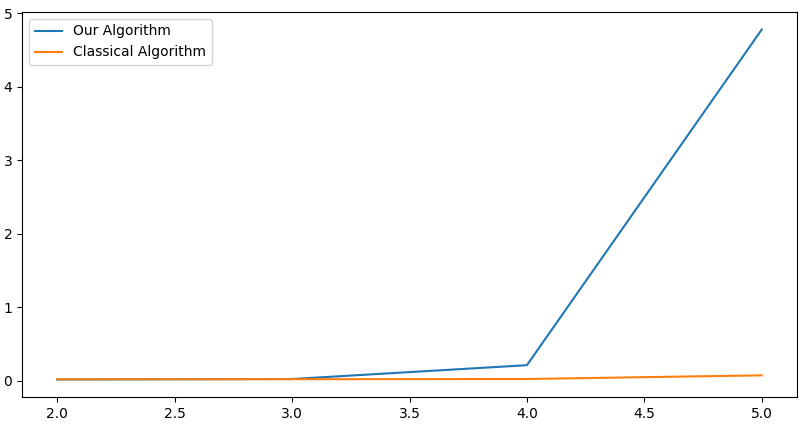
\includegraphics[width=\hsize]{../Docs/Images/expr.png}}
    \caption{Time to compute $\hbox{\tencsc Generate-Expression}(n,n)$}
    \label{fig:expr1}
    \medskip
    \centerline{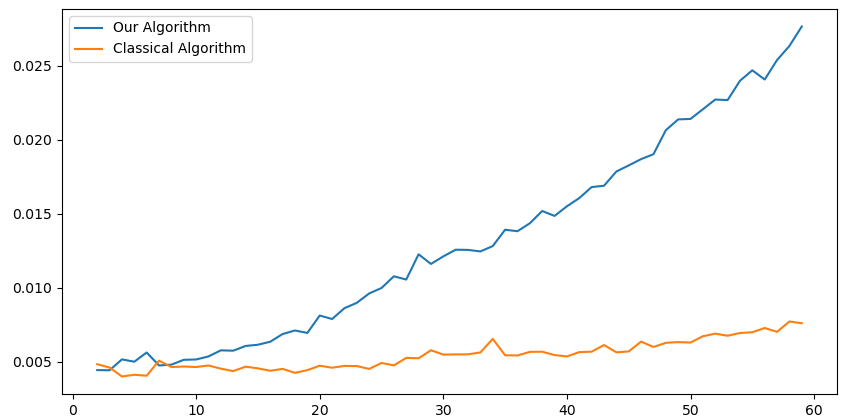
\includegraphics[width=\hsize]{../Docs/Images/expr1.png}}
    \caption{Time to compute $\hbox{\tencsc Generate-Expression}(n,1)$}
    \label{fig:expr2}

\end{figure}

\subsection{Fibonacci}

The fibonacci sequence is a linear recurrence defined by $F_n=F_{n-1}+F_{n-2}$ for $n>1$ and $F_1=F_0=1$.
We wrote a script to compute the $n$th fibonacci number recursively in LLang:

\begin{lstlisting}[language=Caml, frame=single]
fun fib (x) {
    if (x < 2) {
        1
    }{
        (fib (x-1)) + (fib (x-2))
    }
}
let x = (fib n);
_prim_print x
\end{lstlisting}

\noindent Running each implementation 5 times for each $x$, we get the following graph in figure \ref{fig:fib} (as $x$ varies):

\begin{figure}

    \centerline{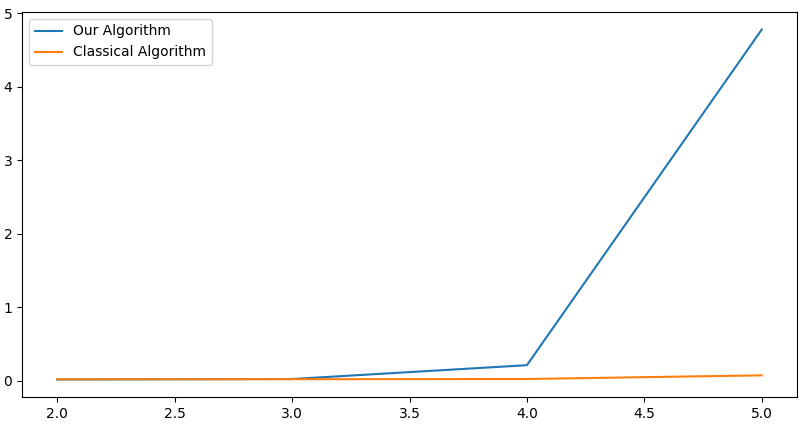
\includegraphics[width=\hsize]{../Docs/Images/expr.png}}
    \caption{Time to compute $\hbox{\tt fib}(x)$}
    \label{fig:fib}

\end{figure}

Our implementation takes approximately $\sim ab^x$ seconds to run where $a=0.000138585, b=1.64685$, and the menhir-based interpreter takes $\sim ab^x$ seconds where $a=0.00000362553, b=1.5809$.

\section{Conclusion}

We can see that linear reduction is significantly slower than the menhir-based interpreter.
This can be for various reasons:
\begin{enumerate}
    \item Linear reduction is an $O(n^2)$-time algorithm (when no reduction produces a string of printable tokens, and every reduction reduces two tokens to one).
        This is because a string of the form $\s s^1_1\s s^2_2\cdots\s s^n_n$ will take $n$ applications of the $\beta$-reducer, each application taking $n-k$ iterations (since $\beta$ is recursive).
        This can be made more efficient: instead of starting the next $\beta$-reduction at the beginning of a string, it can be started at the token before the one just reduced.
        Meaning once $\s s^{n-1}$ and $\s s^n$ are reduced to give $\s x^{n-1}$, we can begin the next iteration of the $\beta$-reducer at $\s s^{n-2}\s x^{n-1}$.
        Unfortunately, implementing this did not lead to substantial increases in efficiency.

    \item When handling function calls, linear reduction simply re-reduces the string in the definition of the function.
        This requires it to parse and interpret the function again.
        But classically, since the function definition has already been parsed and a parse tree created, further parsing of the function is not created.
        This means that classical methods handle function calls better than linear reduction, but on the other hand linear reduction can handle macro-like programming better.
        For example, if one were to change the state to map \ttt( to $\Lbrace$, the menhir-based interpreter would not be able to reparse the function to reinterpret \ttt(.
        But this naturally happens with linear reduction, for better or worse.
        \gobble)\gobble)

    \item The standard methods of parsing code are well-studied and optimized.
        Menhir does not naively parse code, it is an optimized tool.
        Thus comparing a naive implementation of linear reduction to menhir is not a fair comparison.
\end{enumerate}

\end{document}

